\documentclass[tikz, margin=2]{standalone}
\usepackage{amsmath}


\begin{document}
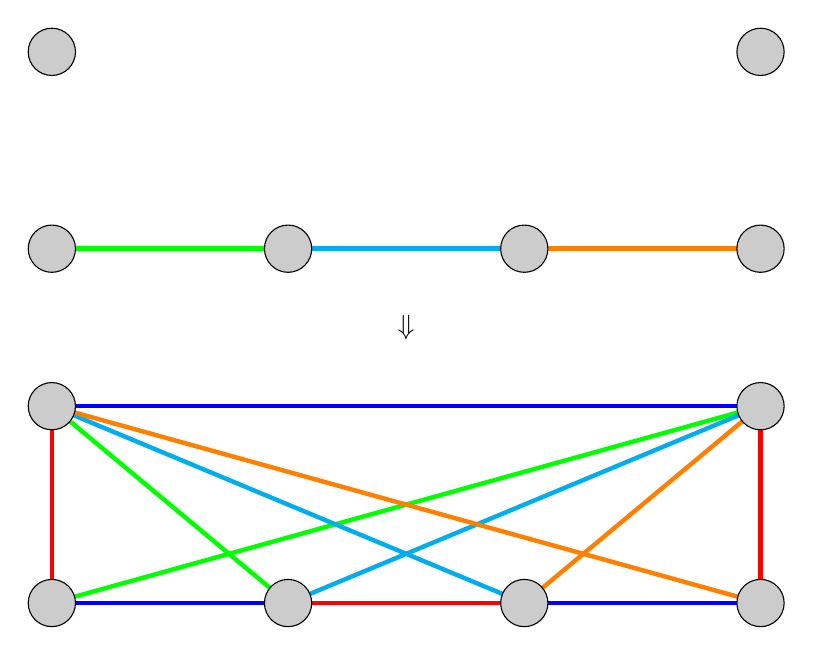
\begin{tikzpicture}

% Draw the initial edge colors
\draw[color=green,ultra thick] (0,0) -- (3,0);
\draw[color=cyan,ultra thick] (3,0) -- (6,0);
\draw[color=orange,ultra thick] (6,0) -- (9,0);
% Draw the inital nodes
\filldraw[color=black,fill=gray!40] (0,2.5) circle (.3);
\filldraw[color=black,fill=gray!40] (9,2.5) circle (.3);
\filldraw[color=black,fill=gray!40] (0,0) circle (.3);
\filldraw[color=black,fill=gray!40] (3,0) circle (.3);
\filldraw[color=black,fill=gray!40] (6,0) circle (.3);
\filldraw[color=black,fill=gray!40] (9,0) circle (.3);

% Arrow down
\node at (4.5,-1) {\(\Downarrow\)};

% Draw the loop
\draw[color=red,ultra thick] (0,-2) -- (0,-4.5);
\draw[color=blue,ultra thick] (0,-4.5) -- (3,-4.5);
\draw[color=red,ultra thick] (3,-4.5) -- (6,-4.5);
\draw[color=blue,ultra thick] (6,-4.5) -- (9,-4.5);
\draw[color=red,ultra thick] (9,-4.5) -- (9,-2);
\draw[color=blue,ultra thick] (0,-2) -- (9,-2);
% Draw to the right
\draw[color=green,ultra thick] (0,-4.5) -- (9,-2);
\draw[color=cyan,ultra thick] (3,-4.5) -- (9,-2);
\draw[color=orange,ultra thick] (6,-4.5) -- (9,-2);
% Draw to the left
\draw[color=green,ultra thick] (3,-4.5) -- (0,-2);
\draw[color=cyan,ultra thick] (6,-4.5) -- (0,-2);
\draw[color=orange,ultra thick] (9,-4.5) -- (0,-2);
% Draw the final nodes
\filldraw[color=black,fill=gray!40] (0,-2) circle (.3);
\filldraw[color=black,fill=gray!40] (9,-2) circle (.3);
\filldraw[color=black,fill=gray!40] (0,-4.5) circle (.3);
\filldraw[color=black,fill=gray!40] (3,-4.5) circle (.3);
\filldraw[color=black,fill=gray!40] (6,-4.5) circle (.3);
\filldraw[color=black,fill=gray!40] (9,-4.5) circle (.3);

\end{tikzpicture}
\end{document}
